\documentclass[12pt,a4paper]{report}

% -------------------------------------------------
% PACKAGES
% -------------------------------------------------
\usepackage[utf8]{inputenc}
\usepackage[T1]{fontenc}
\usepackage{lmodern}
\usepackage[english]{babel}
\usepackage{amsmath, amssymb}
\usepackage{graphicx}
\usepackage{float}
\usepackage{caption}
\captionsetup{font=small, labelfont=bf}
\captionsetup[figure]{position=bottom}
\captionsetup[table]{position=top}
\usepackage{subcaption}
\usepackage{geometry}
\usepackage{booktabs}
\usepackage{algorithm}
\usepackage{algpseudocode}
\usepackage{setspace}
\usepackage{titlesec}
\usepackage{enumitem}
\usepackage{tocloft}
\usepackage{hyperref}
\usepackage[nameinlink, noabbrev]{cleveref}

% -------------------------------------------------
% PAGE FORMAT
% -------------------------------------------------
\geometry{top=2.5cm, bottom=2.5cm, left=2.5cm, right=2.5cm}
\setstretch{1.2}
\setlength{\parskip}{6pt}
\setlength{\parindent}{0pt}
\raggedbottom
\setlength{\emergencystretch}{3em}
\sloppy
\setlist[itemize]{noitemsep, topsep=3pt}
\setlist[enumerate]{noitemsep, topsep=3pt}
\graphicspath{{figures/}}

\hypersetup{
  colorlinks=true,
  linkcolor=black,
  urlcolor=cyan,
  citecolor=blue
}

% Algorithms
\makeatletter
\setlength{\ALG@thistlm}{\leftmargin}
\makeatother

% -------------------------------------------------
% TITLE FORMAT
% -------------------------------------------------
\titleformat{\chapter}[hang]
  {\normalfont\huge\bfseries}
  {\thechapter.}{1em}{}
\titlespacing*{\chapter}{0pt}{-10pt}{10pt}

\titleformat{\section}
  {\normalfont\bfseries\large}{\thesection.}{0.5em}{}

\titleformat{\subsection}
  {\normalfont\bfseries\normalsize}{\thesubsection.}{0.5em}{}

% -------------------------------------------------
% TABLE OF CONTENTS
% -------------------------------------------------
\renewcommand{\cftbeforetoctitleskip}{-1em}
\renewcommand{\cftaftertoctitleskip}{1em}
\setlength{\cftchapindent}{0pt}
\setlength{\cftsecindent}{1.5em}
\setlength{\cftsubsecindent}{3em}
\setlength{\cftsubsubsecindent}{4.5em}
\renewcommand{\cftdotsep}{1}
\addto\captionsenglish{\renewcommand{\bibname}{References}}

\begin{document}
% -------------------------------------------------
% COVER PAGE
% -------------------------------------------------
\begin{titlepage}
    \centering
    
\includegraphics[width=0.35\textwidth]{logo_ulpgc.png} \\[0.8cm]

    {\huge \textbf{Big Data}} \\[0.3cm]
    {\Large Degree in Data Science and Engineering} \\[0.2cm]
    {\large School of Computer Engineering} \\[0.2cm]
    {\large Academic year 2026--2027} \\[1cm]

    \line(1,0){400} \\[4mm]
    {\Huge \textbf{Individual Assignment 3}} \\[3mm]
    {\LARGE Parallel Matrix Multiplication} \\[3mm]
    {\large \textit{How does the number of threads affect speedup and efficiency\\on a hybrid processor?}} \\[4mm]
    \line(1,0){400} \\[1cm]

    {\large
    \begin{tabular}{l}
        \textbf{Name} \\
        \midrule
        Claudia Álvarez González \\
    \end{tabular}} \\[1cm]

    {\large \textbf{Repository:} \url{https://github.com/Claudia1771/bigdata-matrix-multiplication}} \\[2mm]
    {\normalsize (folder \texttt{assignment3})}

    \vfill

    {\large \today}
\end{titlepage}

% -------------------------------------------------
% INDEXES
% -------------------------------------------------
\pagenumbering{roman}
\tableofcontents
\newpage
\listoffigures
\newpage
\listoftables
\newpage
\listofalgorithms
\newpage
\pagenumbering{arabic}

% =================================================
\chapter*{Abstract}
\addcontentsline{toc}{chapter}{Abstract}
% =================================================

This study parallelises the blocked matrix multiplication of Assignment~2 with OpenMP and measures how its time,
speedup $S(p) = T_{\text{seq}}/T_p$ and efficiency $E(p) = S(p)/p$ change with the number of threads $p$ on a hybrid
laptop processor (6 performance cores with two hardware threads each, plus 10 efficient cores). The parallel version
distributes rows of blocks among the threads, needs no synchronisation, uses exactly the same kernel as the
sequential baseline and produces bit-identical results. Each thread count was run with an affinity mask that adds,
in turn, physical performance cores, their hyper-threads, the efficient cores and 2$\times$ oversubscription; the 34
configurations ran in a random order on AC power, with five repetitions each. The parallel overhead with one thread
was at most 6\%. With one thread per performance core ($p = 6$) the speedup was 4.8 for $n = 1024$ and $2048$
(efficiency 0.79) but only 2.9 for $n = 4096$, whose long runs made the clock of each core fall from 3.95~GHz with one
active thread to about 2.2~GHz with six. Hyper-threads added nothing, the efficient cores raised the speedup only for
$n = 2048$ (to 6.5 with 22 threads), oversubscription brought no consistent gain, and the static and dynamic
schedules differed by less than 10\%. Memory did not depend on $p$. The results show that on this laptop the power
budget shared by all cores, not the algorithm, is the main limit to parallel speedup; they are limited to the tested
implementation and machine.

% =================================================
\chapter{Introduction and Objective}
% =================================================

Assignment~2 showed that cache blocking is the fastest sequential dense method among those tested, with an almost
constant cost per operation up to $n = 4096$~\cite{a2}. A single core, however, uses only a small part of a modern
processor. This study parallelises that blocked method with OpenMP~\cite{openmp52} and measures how its performance
changes with the number of threads on a laptop processor that combines fast performance cores (P-cores), each with
two hardware threads, and slower efficient cores (E-cores).

\section{Research question}

\textit{How does the number of threads $p$ affect the execution time, speedup and efficiency of a shared-memory
parallel version of the blocked matrix multiplication, and when does adding threads stop helping on a hybrid
processor?}

The factors changed are the number of threads $p \in \{1, 2, 4, 6, 8, 12, 16, 22, 44\}$, the matrix size
$n \in \{1024, 2048, 4096\}$ and, in a secondary experiment, the loop schedule (static or dynamic). The outcomes are
the execution time, the speedup $S(p)$, the efficiency $E(p)$ and the peak memory.

\section{Hypotheses}

Stated before running the experiment:
\begin{enumerate}[label=\textbf{H\arabic*.}]
  \item The speedup is close to linear while each thread has its own performance core ($p \le 6$), because the
  blocked kernel is compute-bound and the threads do not share data that they write.
  \item The second hardware thread of each P-core ($7 \le p \le 12$) adds little, because the two threads share the
  execution units of the core.
  \item Adding the efficient cores ($p > 12$) still increases the speedup, but the efficiency drops; with cores of
  different speed, a dynamic schedule is better than a static one.
  \item More threads than logical processors ($p = 44$) give no further gain.
  \item Larger matrices give a higher speedup, because the fixed parallel overheads are amortised over more work, and
  the memory does not depend on $p$.
\end{enumerate}

% =================================================
\chapter{Background}
% =================================================

\section{Speedup, efficiency and Amdahl's law}

Let $T_{\text{seq}}(n)$ be the time of the sequential baseline and $T_p(n)$ the time of the parallel version with
$p$ threads for the same input. The speedup is $S(p) = T_{\text{seq}}(n) / T_p(n)$ and the efficiency is
$E(p) = S(p)/p$. If a fraction $f$ of the work cannot be parallelised, Amdahl's law bounds the speedup by
$S(p) \le 1 / \left(f + (1-f)/p\right)$~\cite{amdahl1967}; with a fixed time budget, larger problems usually have a
smaller serial fraction and scale better~\cite{gustafson1988}. On real hardware, the speedup is also limited by
shared resources: memory bandwidth and the shared L3 cache, the execution units shared by two hardware threads of
the same core (simultaneous multithreading), and, on a hybrid processor, the different speed of the
cores~\cite{hennessy2017}.

\section{Parallelising the blocked multiplication}

In the blocked method the result $C$ is divided into rows of $b \times b$ blocks. Each block row of $C$ depends on
the corresponding rows of $A$ and on all of $B$, which are only read. Different block rows can therefore be computed
independently by different threads without locks: each thread writes only to its own rows of $C$
(\Cref{alg:par}). Inside a block row the order of the operations is the same as in the sequential method, so every
element $C_{ij}$ still adds its products in increasing order of $k$ and the result is bit-identical for any number of
threads. OpenMP distributes the iterations of the outer loop either statically, in equal contiguous shares decided in
advance, or dynamically, handing one block row at a time to the next idle thread~\cite{openmp52}; the dynamic schedule
adapts to threads that run at different speeds.

\begin{algorithm}[H]
\caption{Parallel blocked multiplication (rows of blocks distributed among threads)}
\label{alg:par}
\begin{algorithmic}[1]
\Require $A, B \in \mathbb{R}^{n \times n}$, block size $b$, $p$ threads
\State $C \gets 0$
\ForAll{block rows $r = 0, 1, \dots, \lceil n/b \rceil - 1$ \textbf{in parallel} (dynamic schedule)}
  \For{$k_0 \gets 0$ \textbf{to} $n-1$ \textbf{step} $b$}
    \For{$j_0 \gets 0$ \textbf{to} $n-1$ \textbf{step} $b$}
      \For{$i \gets rb$ \textbf{to} $\min(rb + b, n) - 1$}
        \For{$k \gets k_0$ \textbf{to} $\min(k_0 + b, n) - 1$}
          \For{$j \gets j_0$ \textbf{to} $\min(j_0 + b, n) - 1$} \State $C_{ij} \gets C_{ij} + A_{ik} B_{kj}$ \EndFor
        \EndFor
      \EndFor
    \EndFor
  \EndFor
\EndFor
\end{algorithmic}
\end{algorithm}

% =================================================
\chapter{Methodology}
\label{chap:method}
% =================================================

\section{Implementations}

Both methods are in \texttt{src/parallel.c}, compiled with GCC 16.2.0 and \texttt{-O2 -std=c11 -fopenmp}.
\begin{itemize}
  \item \texttt{seq}, the sequential baseline: the blocked method of Assignment~2 ($b = 64$), processing the block
  rows in order.
  \item \texttt{par}, the parallel method: the same block rows distributed among an OpenMP team
  (\texttt{\#pragma omp parallel for schedule(dynamic, 1)}, or \texttt{schedule(static)} in the schedule
  experiment).
\end{itemize}
Both methods call the same function \texttt{block\_row}, which contains the whole kernel and is compiled once, so they
differ only in how the block rows are distributed. A first version that inlined the kernel inside the OpenMP loop was
discarded: the compiler vectorised the kernel of \texttt{seq} but not the one generated for \texttt{par}, which made
the parallel method twice as slow with one thread (0.54~s against 0.26~s for $n = 1024$) and would have biased every
speedup. With the shared kernel (and \texttt{restrict} pointers, valid because $C$ is a new allocation) the GCC
vectorisation report confirms a single vectorised copy of the inner loop. The number of threads is set with
\texttt{omp\_set\_num\_threads} and \texttt{OMP\_DYNAMIC=false}; every measurement prints the size of the team that
was actually created. No numerical library is used, so there are no hidden library threads.

\section{Inputs and correctness}

The inputs are the dense matrices of Assignments~1 and~2 (NumPy PCG64 with seed $42+n$, uniform \texttt{float64}
values in $[0,1)$), read from the same files. Before benchmarking, \texttt{verify.py} ran 156 tests: known products
($1\times1$, $2\times2$, $AI = A$, $A\,0 = 0$) and random matrices with
$n \in \{1, 2, 3, 17, 64, 100, 129, 300\}$ (sizes that are not multiples of the block, or with fewer block rows than
threads) for $p \in \{1, 2, 3, 7, 22, 44\}$ and both schedules, compared with \texttt{numpy.matmul}
($\mathrm{rtol} = \mathrm{atol} = 10^{-12}$) and bit by bit with \texttt{seq}. All passed. During the benchmark every
multiplication returns a checksum of the result.

\section{Thread placement}

The processor (Intel Core Ultra 7 155H) has 6 P-cores with two hardware threads each, 8 E-cores and 2 low-power
E-cores: 16 physical cores and 22 logical processors. Running two CPU-bound processes pinned to two logical
processors showed which pairs share a physical P-core: (0,\,1), (10,\,11), (12,\,13), (14,\,15), (16,\,17) and
(18,\,19); each process becomes twice as slow only when both share a core. Every configuration was started with an
affinity mask chosen according to $p$ (\Cref{tab:affinity}), so that the results separate the effect of physical
cores, hyper-threads, efficient cores and oversubscription.

\begin{table}[H]
\centering
\small
\caption{Affinity plan: logical processors that each configuration may use.}
\label{tab:affinity}
\begin{tabular}{lll}
\toprule
\textbf{Configuration} & \textbf{Logical processors} & \textbf{What it adds} \\
\midrule
\texttt{seq}, \texttt{par} with $p = 1$ & 12 & One performance core \\
$p = 2, 4, 6$ & 12, 0, 10, 14, 16, 18 (first $p$) & One thread per physical P-core \\
$p = 8, 12$ & + 13, 1, 11, 15, 17, 19 (first $p-6$) & Hyper-thread siblings \\
$p = 16, 22$ & all 22 & Efficient and low-power cores \\
$p = 44$ & all 22 & 2$\times$ oversubscription \\
\bottomrule
\end{tabular}
\end{table}

\section{Measurement protocol}

The protocol of the previous assignments is reused: each configuration runs in a fresh process with \texttt{HIGH}
priority, one warm-up and five measured repetitions, and budgets of 300~s per multiplication and 4~GiB per process.
Two changes were made after a first complete run in a fixed order (sequential first, then increasing $p$, kept in
\texttt{results/preliminary\_fixed\_order}). In that run the laptop became slower under sustained load: running the
same $n = 4096$ configurations again in the order parallel ($p=1$), sequential, parallel ($p=1$) gave 13.0, 13.5 and
15.0~s, and the static and dynamic schedules with $p = 6$ gave 0.37~s each in one round and 0.60~s each in the next.
A fixed order therefore favours the configurations that run first. In the reported run the 34 configurations are
executed in a random order (seed 2026, recorded as \texttt{order} in \texttt{runs.csv}), each one after an idle period
of 20~s, and the effective clock of logical processor~12, which belongs to every affinity mask, is recorded during
each configuration. The timer covers only the multiplication (allocation of $C$, thread start-up and the parallel loop); it uses
\texttt{clock\_gettime(CLOCK\_MONOTONIC)}, because \texttt{omp\_get\_wtime} has only millisecond resolution on this
platform. Medians and interquartile ranges (IQR) are reported~\cite{hoefler2015}, and $S(p)$ and $E(p)$ are computed
from the medians. Memory is the peak working set of the process. The harness refuses to start on battery: a test on
battery showed the sequential time for $n = 2048$ rising from 2.1~s in the first multiplication to 4.7~s in the
second, as the laptop reduced its power after a few seconds, which would have inflated every speedup. For every
configuration it records whether the laptop stayed on AC power and the utilisation of the allowed logical processors
and of the others.

\section{Environment}

\begin{table}[H]
\centering
\small
\caption{Hardware and software environment of the reported run.}
\label{tab:env}
\begin{tabular}{lp{10.5cm}}
\toprule
\textbf{Item} & \textbf{Value} \\
\midrule
CPU & Intel Core Ultra 7 155H: 6 P-cores (2 threads each), 8 E-cores, 2 LP E-cores; 24~MB L3 \\
Cores / logical processors & 16 / 22 \\
RAM & 16 GB \\
Operating system & Windows 11, \textit{Best performance} power mode, on AC power \\
Compiler & GCC 16.2.0 (MinGW-w64 UCRT), \texttt{-O2 -std=c11 -fopenmp}, libgomp \\
Threads & \texttt{omp\_set\_num\_threads(p)}, \texttt{OMP\_DYNAMIC=false}; affinity as in \Cref{tab:affinity} \\
\bottomrule
\end{tabular}
\end{table}

% =================================================
\chapter{Results}
\label{chap:results}
% =================================================

All values come from \texttt{results/raw\_measurements.csv}, \texttt{runs.csv}, \texttt{summary.csv},
\texttt{speedup.csv} and \texttt{schedule.csv}, produced by \texttt{analyze.py}. Speedup and efficiency are computed
from the medians.

\section{Correctness and execution conditions}

Every one of the 34 configurations was executed on AC power, every repetition produced the same checksum for a given
$n$ whatever the thread count or schedule, and every parallel run obtained the requested team size. The utilisation of
the logical processors outside each affinity mask was at most 12\%.

\section{Sequential baseline and parallel overhead}

The sequential baseline took 0.198~s ($n = 1024$), 1.591~s ($n = 2048$) and 17.33~s ($n = 4096$). The parallel method
with one thread took 0.196~s, 1.687~s and 18.05~s, i.e.\ 0.99, 1.06 and 1.04 times the baseline: the cost of the OpenMP
machinery is at most 6\%, within the variability of the runs.

\section{Speedup and efficiency}

\begin{table}[H]
\centering
\small
\caption{Speedup $S(p) = T_{\text{seq}} / T_p$ (medians, 5 repetitions) and, below, efficiency $E(p) = S(p)/p$.
Columns 2--6: one thread per performance core; 8--12: plus hyper-threads; 16--22: plus efficient cores; 44: 2$\times$
oversubscription.}
\label{tab:speedup}
\resizebox{\textwidth}{!}{%
\begin{tabular}{l rrrrrrrrr}
\toprule
$n$ & $p = 1$ & 2 & 4 & 6 & 8 & 12 & 16 & 22 & 44 \\
\midrule
\multicolumn{10}{l}{\textit{Speedup}} \\
1024 & 1.01 & 2.03 & 3.43 & 4.78 & 4.73 & 4.22 & 4.31 & 4.44 & 3.40 \\
2048 & 0.94 & 1.77 & 3.20 & 4.74 & 4.65 & 4.53 & 6.36 & 6.48 & 6.61 \\
4096 & 0.96 & 1.38 & 2.55 & 2.90 & 2.92 & 3.23 & 3.41 & 2.95 & 4.01 \\
\midrule
\multicolumn{10}{l}{\textit{Efficiency}} \\
1024 & 1.01 & 1.01 & 0.86 & 0.80 & 0.59 & 0.35 & 0.27 & 0.20 & 0.08 \\
2048 & 0.94 & 0.88 & 0.80 & 0.79 & 0.58 & 0.38 & 0.40 & 0.29 & 0.15 \\
4096 & 0.96 & 0.69 & 0.64 & 0.48 & 0.36 & 0.27 & 0.21 & 0.13 & 0.09 \\
\bottomrule
\end{tabular}}
\end{table}

\begin{figure}[H]
\centering
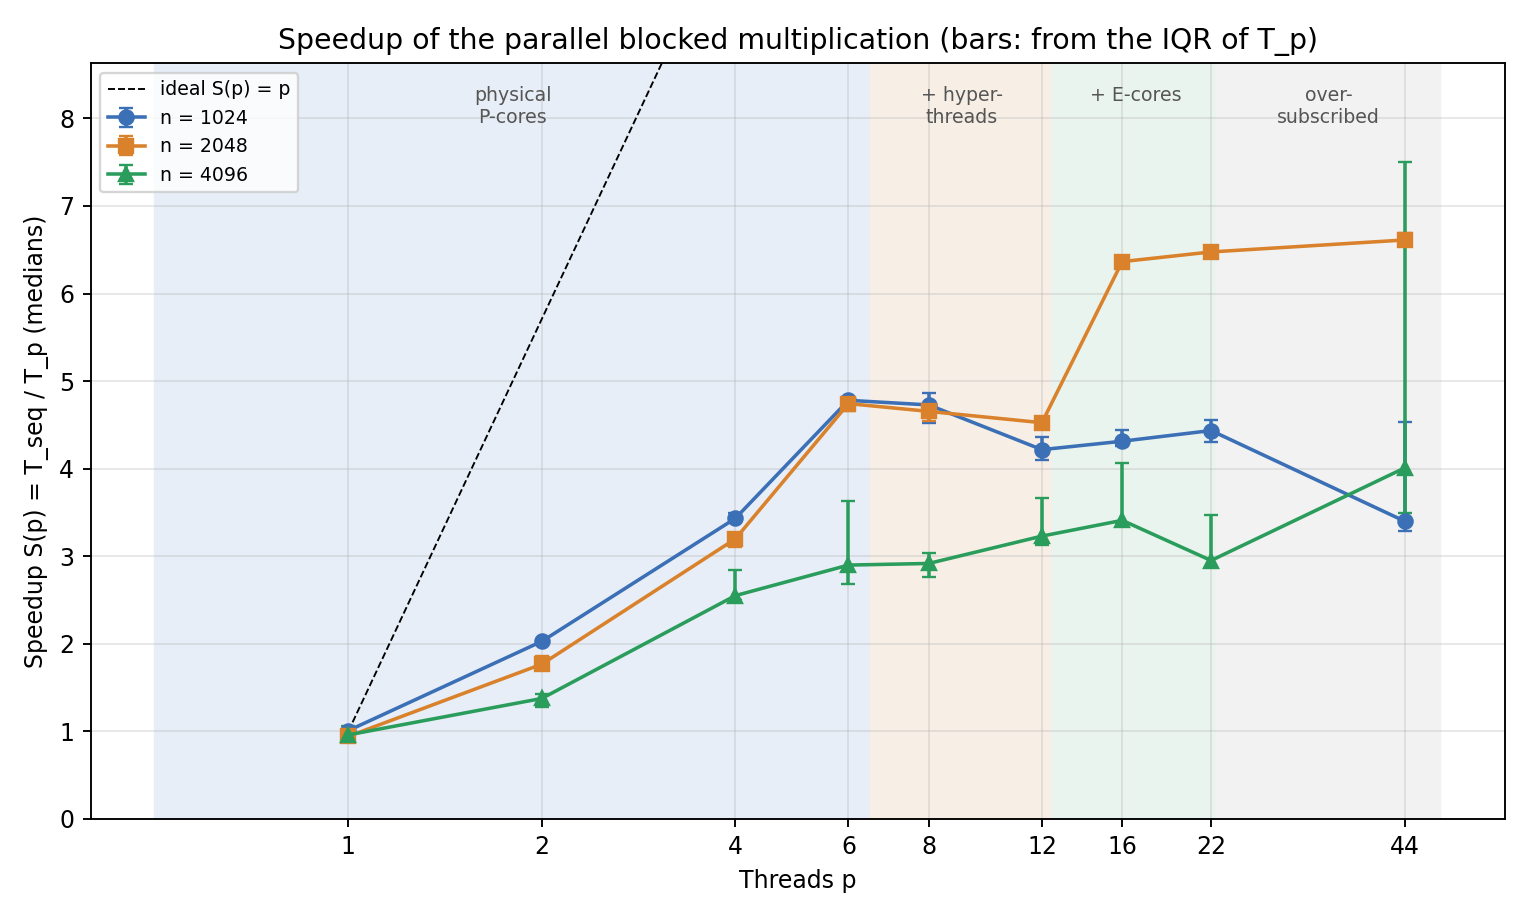
\includegraphics[width=0.92\textwidth]{fig1_speedup.png}
\caption{Speedup versus threads. The shaded regions show what each step of the affinity plan adds; the bars come from
the interquartile range of $T_p$; the dashed line is the ideal $S(p) = p$.}
\label{fig:speedup}
\end{figure}

\begin{figure}[H]
\centering
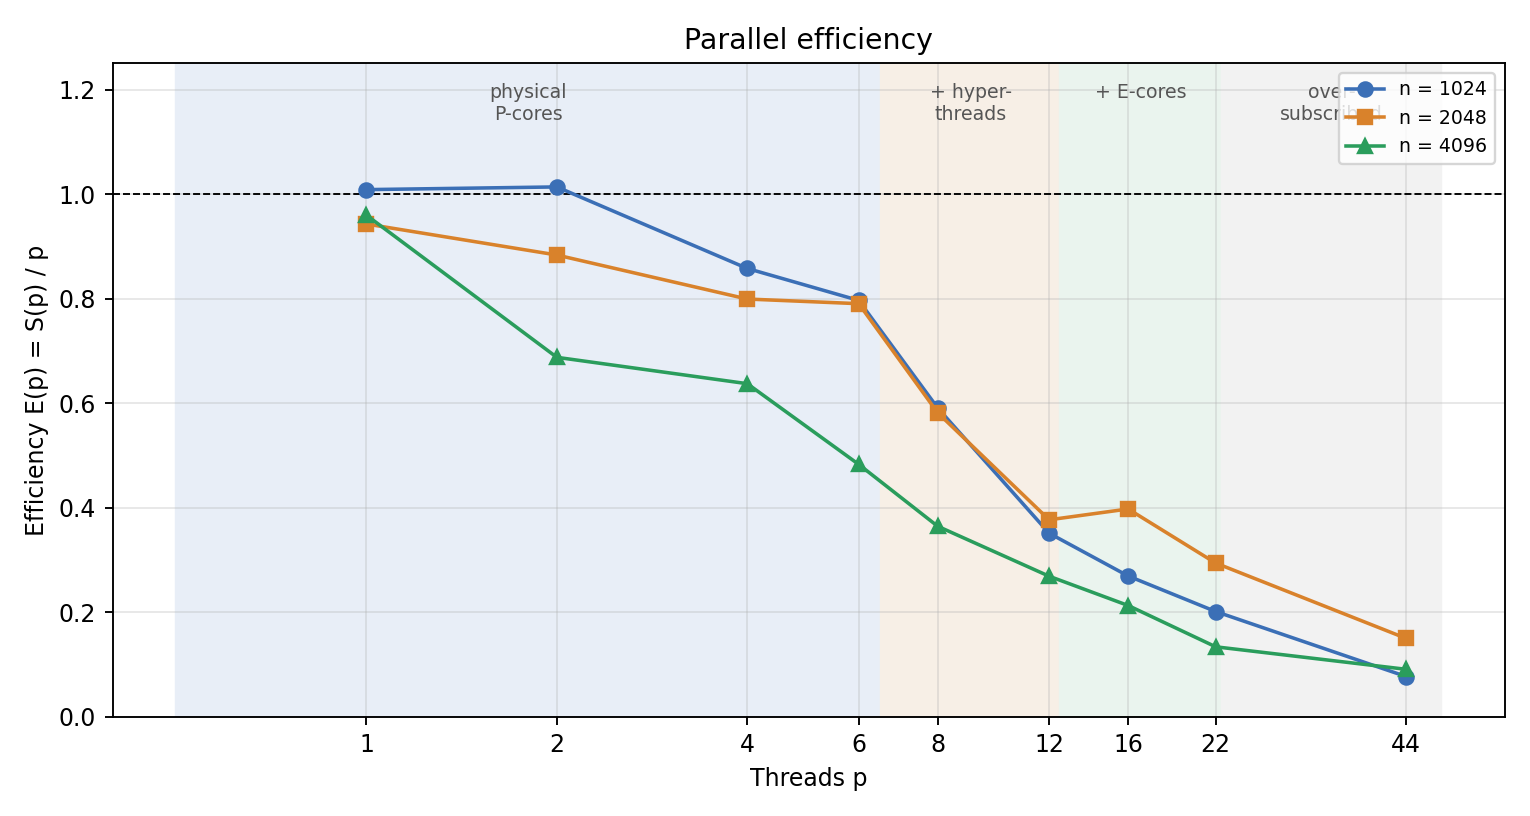
\includegraphics[width=0.85\textwidth]{fig2_efficiency.png}
\caption{Parallel efficiency $E(p) = S(p)/p$.}
\label{fig:efficiency}
\end{figure}

\Cref{tab:speedup} and \Cref{fig:speedup,fig:efficiency} show four distinct regions:
\begin{itemize}
  \item \textbf{Physical performance cores ($p \le 6$).} The speedup grows with every core but stays below the ideal
  line: 4.8 with six threads for $n = 1024$ and $2048$ (efficiency 0.79--0.80), and only 2.9 for $n = 4096$ (0.48).
  \item \textbf{Hyper-threads ($p = 8, 12$).} No gain: the speedup stays at, or slightly below, its value at $p = 6$.
  \item \textbf{Efficient cores ($p = 16, 22$).} A clear gain only for $n = 2048$, from 4.5 to 6.4--6.5; for
  $n = 1024$ and $4096$ the speedup stays between 4.2--4.4 and 2.9--3.4.
  \item \textbf{Oversubscription ($p = 44$).} No consistent effect: worse for $n = 1024$ (3.4), unchanged for
  $n = 2048$ (6.6) and higher but very variable for $n = 4096$ (4.0, IQR 61\%).
\end{itemize}
The highest speedup was 6.6 ($n = 2048$, $p = 44$, practically equal to $p = 22$).

\begin{figure}[H]
\centering
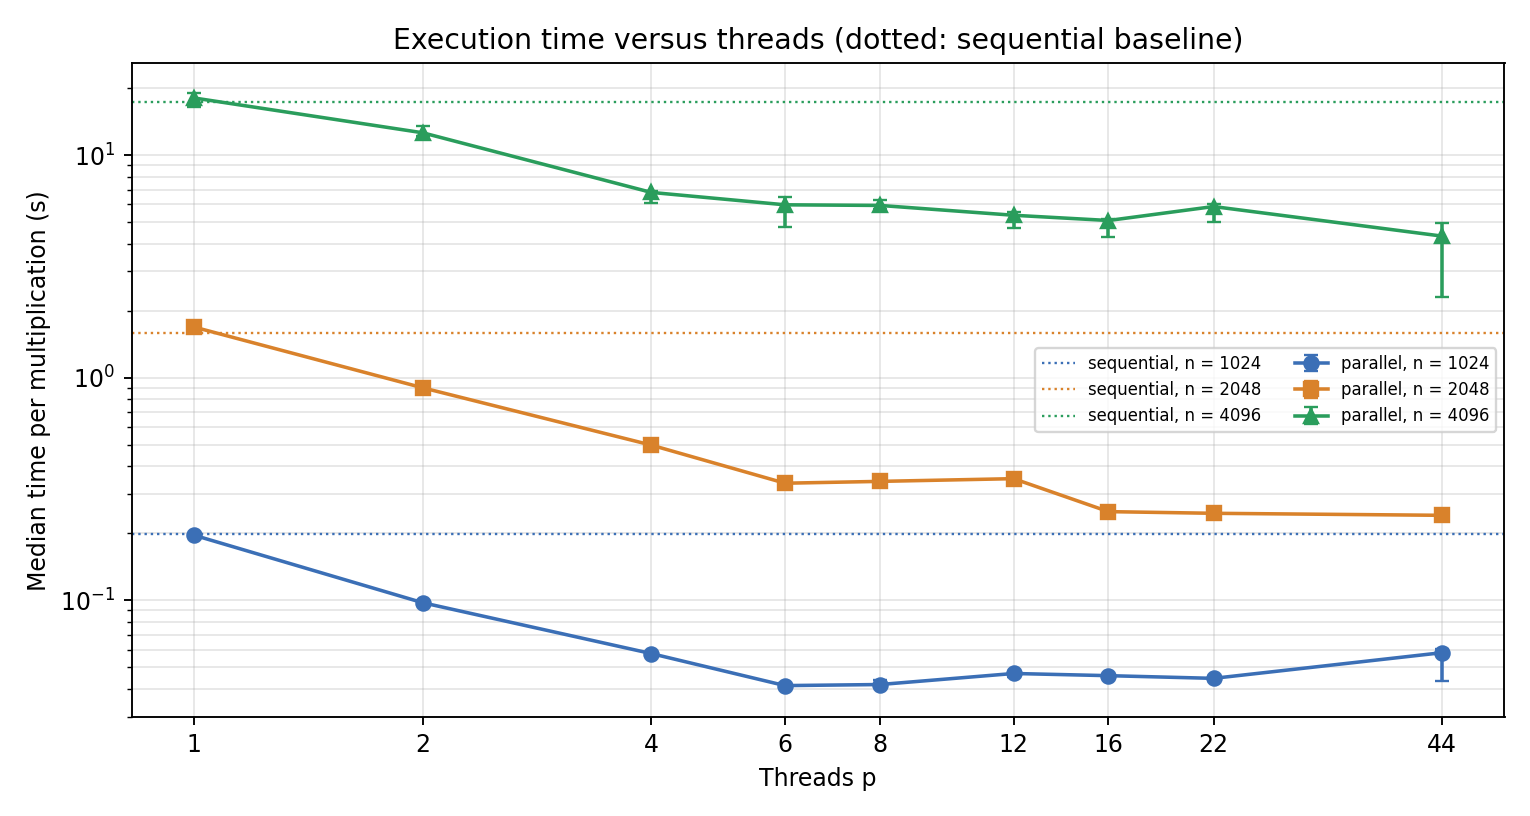
\includegraphics[width=0.85\textwidth]{fig3_time.png}
\caption{Median time per multiplication versus threads (bars: IQR; dotted lines: sequential baseline).}
\label{fig:time}
\end{figure}

\section{Clock frequency}

\begin{figure}[H]
\centering
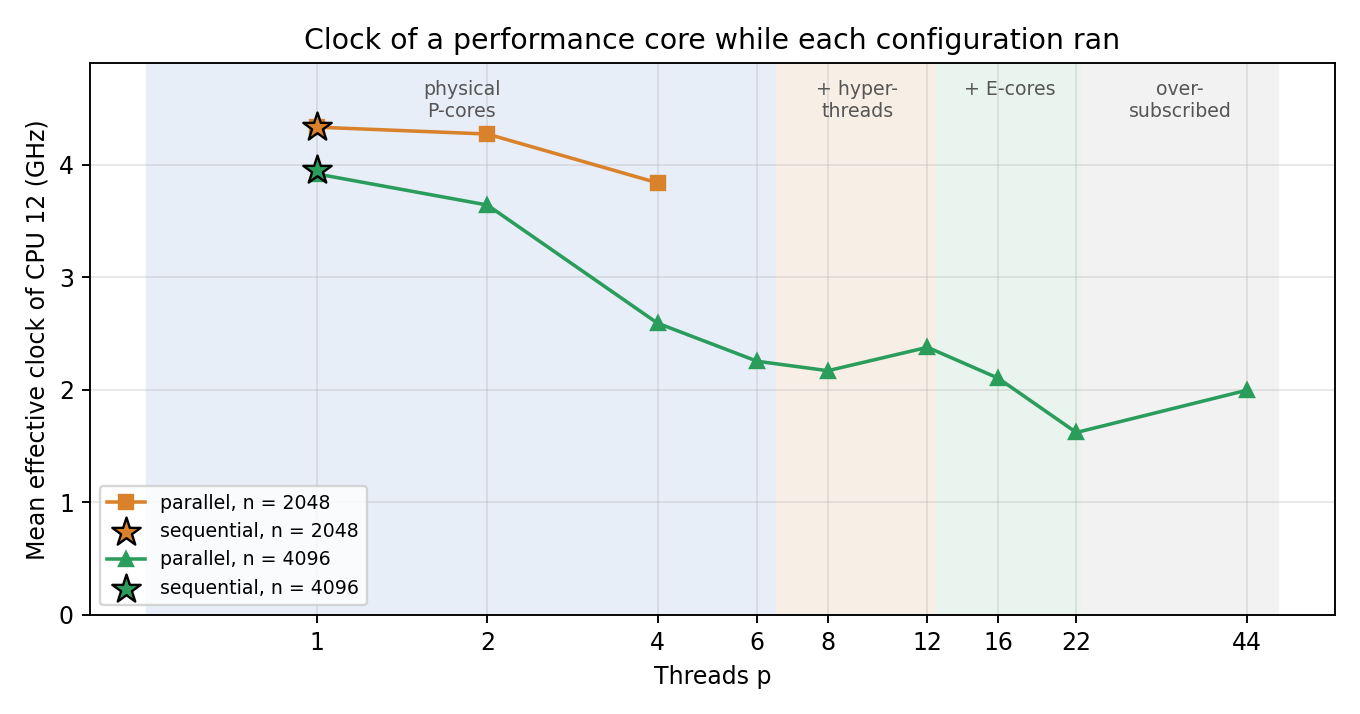
\includegraphics[width=0.85\textwidth]{fig6_clock.png}
\caption{Mean effective clock of logical processor~12 (a performance core present in every mask) during each
configuration. The counter is sampled every 0.5~s, so only configurations long enough to be sampled appear.}
\label{fig:clock}
\end{figure}

For $n = 4096$, whose configurations last between 22 and 108~s, the clock of the performance core fell from 3.95~GHz
with one active thread to 3.64~GHz with two, 2.59~GHz with four and 2.25~GHz with six threads, and to 1.6--2.4~GHz
with more threads (\Cref{fig:clock}). For $n = 2048$, whose configurations last a few seconds, it stayed at
4.3~GHz with one or two threads and 3.8~GHz with four.

\section{Variability}

For $n = 1024$ and $2048$ the IQR is below 9\% of the median in all configurations except $p = 44$ with $n = 1024$
(28\%). For $n = 4096$ it is between 9\% and 28\%, and 61\% for $p = 44$: the long runs are the ones exposed to the
changes of clock frequency. Every parallel run obtained exactly the requested number of threads.

\section{Static versus dynamic schedule}

\begin{table}[H]
\centering
\small
\caption{Median time (s) for $n = 2048$ with the two schedules (5 repetitions each).}
\label{tab:schedule}
\begin{tabular}{rrrr}
\toprule
$p$ & \textbf{dynamic} & \textbf{static} & \textbf{static / dynamic} \\
\midrule
6  & 0.335 & 0.364 & 1.09 \\
12 & 0.352 & 0.373 & 1.06 \\
16 & 0.250 & 0.234 & 0.94 \\
22 & 0.246 & 0.258 & 1.05 \\
\bottomrule
\end{tabular}
\end{table}

The two schedules differ by less than 10\%, in both directions (\Cref{tab:schedule}, \Cref{fig:schedule}).

\begin{figure}[H]
\centering
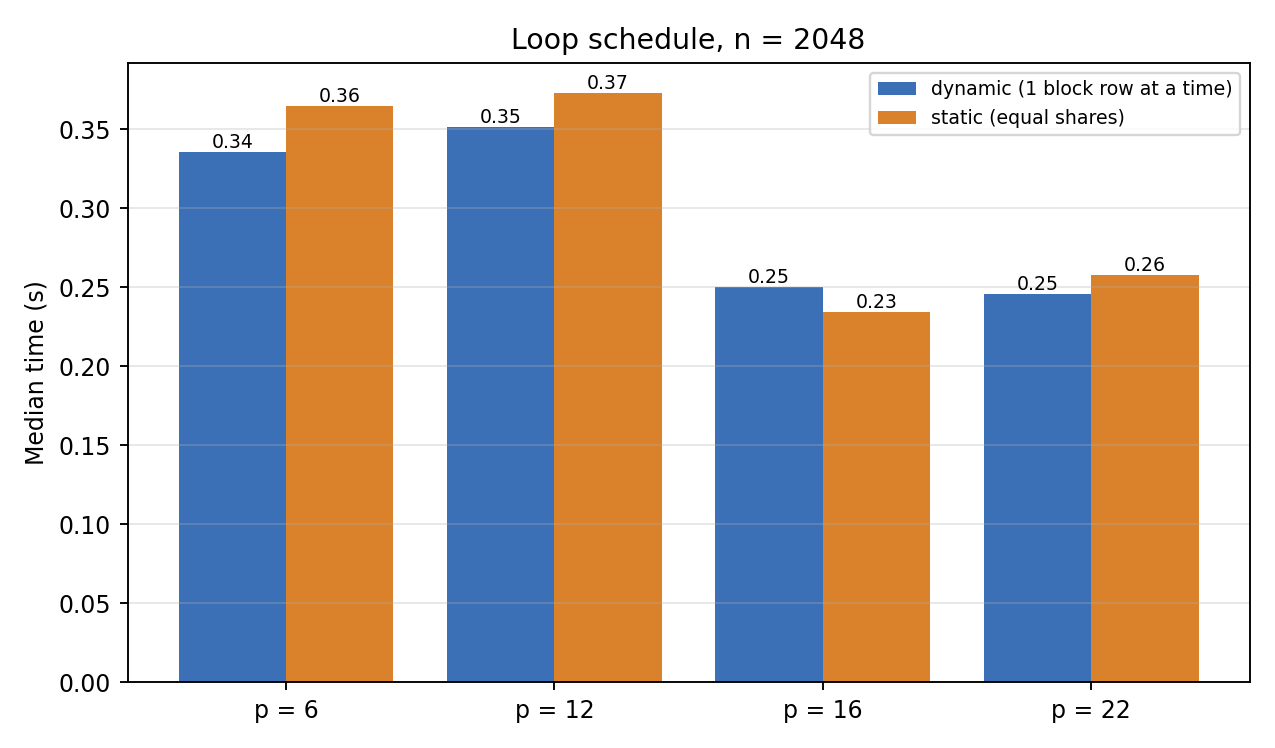
\includegraphics[width=0.7\textwidth]{fig4_schedule.png}
\caption{Static versus dynamic schedule, $n = 2048$.}
\label{fig:schedule}
\end{figure}

\section{Memory}

The peak working set did not depend on the number of threads: 28.3--29.6~MiB for $n = 1024$, 100.3--101.6~MiB for
$n = 2048$ and 388.3--389.6~MiB for $n = 4096$ (\Cref{fig:memory}), essentially the three matrices ($24n^2$ bytes).
The parallel version adds only the thread stacks, about 1~MiB for 44 threads.

\begin{figure}[H]
\centering
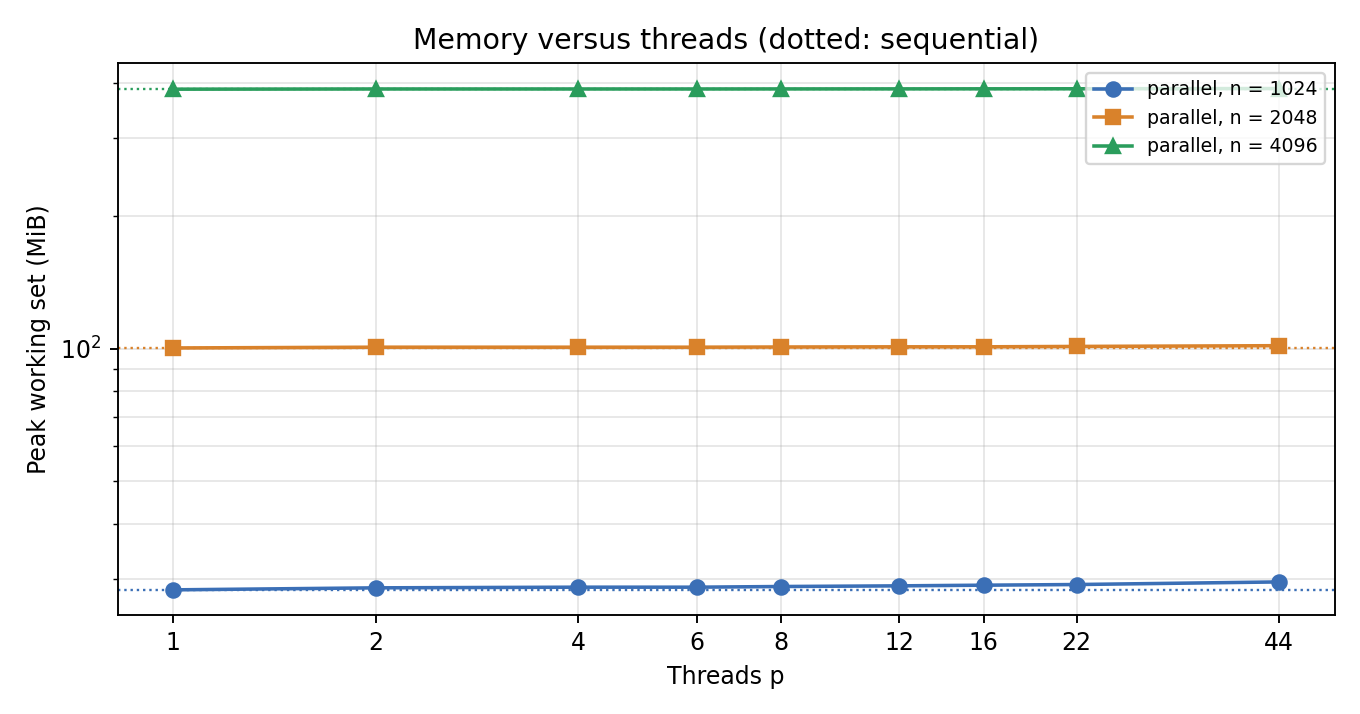
\includegraphics[width=0.8\textwidth]{fig5_memory.png}
\caption{Peak working set versus threads (dotted lines: sequential baseline).}
\label{fig:memory}
\end{figure}

% =================================================
\chapter{Discussion}
% =================================================

\section{Why the speedup is sublinear on the performance cores (H1)}

\textbf{H1 is not supported.} With one thread per performance core the speedup was 4.8 instead of 6 for the two
smaller sizes and 2.9 for $n = 4096$. The parallel overhead itself is small (at most 6\% with one thread) and the
threads never wait for each other, so the main limit is the hardware. The clock measurements point to the power
budget of the laptop: all the cores share one power limit, so the more cores are active, the lower the frequency of
each one. For $n = 4096$ the clock of a performance core fell to 2.25~GHz with six threads. If each core is
$3.95/2.25 \approx 1.75$ times slower than in the sequential run, the best possible speedup with six cores is about
$6 / 1.75 \approx 3.4$; the measured 2.9 is close to this bound. The configurations of $n = 2048$ last only a few
seconds, and laptops typically allow a higher power for short bursts before falling to a lower sustained
limit~\cite{hennessy2017}; this is consistent with the higher clock (3.8--4.3~GHz) and the better speedup measured for
that size. The remaining gap can be explained by shared resources, mainly the L3 cache and memory bandwidth used to
read $B$, which is read once per block row and does not fit in the 24~MB L3 for $n \ge 2048$. Without hardware
counters this last part cannot be quantified.

\section{Hyper-threads, efficient cores and oversubscription (H2--H4)}

\textbf{H2 is supported.} The second hardware thread of each performance core added nothing. The blocked kernel is
vectorised and keeps the floating-point units of the core busy, and two threads on one core share those units and its
caches, so they can only overlap a small amount of waiting~\cite{hennessy2017}.

\textbf{H3 is only partially supported.} The efficient cores raised the speedup from 4.5 to 6.4 for $n = 2048$, but
not for the other sizes. For $n = 1024$ the matrix has only 16 block rows, so with 16 or more threads each thread gets
at most one row (about 12~ms of sequential work), and the slowest thread and the parallel start-up dominate. For $n = 4096$ the
extra cores mainly lower the shared power budget, and the clock of the performance cores fell to 1.6--2.1~GHz. The
expected advantage of the dynamic schedule on cores of different speed was not observed: the two schedules differed by
less than 10\% in both directions, within the variability of the measurements. With only 32 block rows for 16--22
threads, both schedules leave some threads idle at the end, and the difference between them is smaller than the
effects of frequency.

\textbf{H4 is supported.} With 44 threads on 22 logical processors there was no consistent gain: the result was worse
for $n = 1024$, the same for $n = 2048$, and higher but with a 61\% IQR for $n = 4096$, which does not support a real
improvement.

\section{Problem size and memory (H5)}

\textbf{H5 is only partially supported.} The memory was the same for every thread count, as expected, because the
threads share the three matrices and only add their stacks. However, the largest matrix did not give the highest
speedup: $n = 2048$ scaled best (6.5) and $n = 4096$ worst (2.9--4.0). On this laptop the duration of the run, through
the power limits, mattered more than the amortisation of the parallel overheads, which are already negligible for
$n = 1024$.

\section{Lessons about the experimental design}

Two problems found during the study would have produced wrong conclusions. First, when the kernel was written inside
the OpenMP loop, the compiler vectorised the sequential version but not the parallel one, which made the parallel
method twice as slow with one thread; a fair comparison needs exactly the same compiled kernel. Second, a fixed
execution order made the configurations run later appear slower because the laptop heated up; in that run the static
schedule seemed 1.75 times slower than the dynamic one, an effect that disappeared when the order was randomised.
Measuring the clock frequency was essential to interpret the results.

\section{Limitations}

\begin{itemize}
  \item One laptop. The power and thermal behaviour of a laptop limits the speedup much more than a desktop or server
  would; the results do not describe the algorithm alone.
  \item The clock was sampled on one logical processor only (number 12) and only for configurations longer than about
  0.5~s; the clock of the efficient cores was not measured.
  \item No hardware performance counters (cache misses, memory bandwidth) were collected, so the role of the shared
  cache and memory is inferred, not measured.
  \item Windows chooses which logical processor each thread runs on within the mask; threads were not pinned
  individually.
  \item Only one parallel strategy (rows of blocks) and one block size were tested, and vectorisation was not
  studied as a separate factor (the optional extension was not undertaken).
\end{itemize}

% =================================================
\chapter{Conclusions}
% =================================================

Within the tested implementation and machine:
\begin{itemize}
  \item Distributing rows of blocks among OpenMP threads gives a correct parallel multiplication that needs no
  synchronisation and adds at most 6\% of overhead with one thread.
  \item The speedup is sublinear even on the six performance cores: 4.8 (efficiency 0.79) for $n = 1024$ and $2048$,
  and 2.9 for $n = 4096$.
  \item The main limit on this laptop is the power budget shared by all the cores: the clock of a performance core fell
  from 3.95~GHz to about 2.2~GHz when six cores worked at the same time during long runs.
  \item Hyper-threads give no benefit for this compute-bound kernel; efficient cores help only for intermediate sizes
  (maximum speedup 6.5--6.6 for $n = 2048$); oversubscription gives no consistent benefit.
  \item The static and dynamic schedules performed within 10\% of each other at the tested sizes.
  \item Memory does not depend on the number of threads.
\end{itemize}
Open questions are the behaviour on a machine with a higher power budget, the direct measurement of cache and memory
traffic, and the distributed execution of Assignment~4, where communication adds a new cost.

% =================================================
\chapter*{AI Usage Statement}
\addcontentsline{toc}{chapter}{AI Usage Statement}
% =================================================

In accordance with the course policy, a generative AI assistant was used to support the planning of the experiment,
the development and debugging of the code and scripts, and the language revision of this report. All the measurements
were executed on the author's computer, and the author checked the code, the results and the references and is
responsible for the conclusions.

% =================================================
\chapter*{Reproducibility Materials}
\addcontentsline{toc}{chapter}{Reproducibility Materials}
% =================================================

All materials are in the folder \texttt{assignment3} of the repository
\url{https://github.com/Claudia1771/bigdata-matrix-multiplication}:
\begin{itemize}
  \item \texttt{src/parallel.c}: the sequential and parallel methods.
  \item \texttt{config.json}: sizes, thread counts, affinity plan, schedules, repetitions, budgets, flags, order seed.
  \item \texttt{scripts/}: \texttt{verify.py}, \texttt{run\_experiment.py}, \texttt{analyze.py} and
  \texttt{common.py}.
  \item \texttt{results/}: correctness tests, raw measurements, run conditions (power, load, clock, order), summaries,
  figures and the preliminary fixed-order run.
  \item \texttt{README.md}: build and run commands; the inputs are generated by
  \texttt{assignment2/scripts/generate\_inputs.py}.
\end{itemize}

% =================================================
% REFERENCES
% =================================================
\begin{thebibliography}{99}
\addcontentsline{toc}{chapter}{References}

\bibitem{a2} C.~Álvarez González, ``Optimized approaches and sparse matrices,'' Big Data, Individual Assignment~2,
Univ. Las Palmas de Gran Canaria, Oct.~2026. [Online]. Available:
\url{https://github.com/Claudia1771/bigdata-matrix-multiplication}

\bibitem{openmp52} OpenMP Architecture Review Board, \textit{OpenMP Application Programming Interface, Version 5.2},
Nov.~2021. [Online]. Available: \url{https://www.openmp.org/specifications/}

\bibitem{amdahl1967} G.~M. Amdahl, ``Validity of the single processor approach to achieving large scale computing
capabilities,'' in \textit{Proc. AFIPS Spring Joint Computer Conf.}, 1967, pp.~483--485.

\bibitem{gustafson1988} J.~L. Gustafson, ``Reevaluating Amdahl's law,'' \textit{Commun. ACM}, vol.~31, no.~5,
pp.~532--533, 1988.

\bibitem{hennessy2017} J.~L. Hennessy and D.~A. Patterson, \textit{Computer Architecture: A Quantitative Approach},
6th~ed. Cambridge, MA, USA: Morgan Kaufmann, 2017.

\bibitem{hoefler2015} T.~Hoefler and R.~Belli, ``Scientific benchmarking of parallel computing systems: Twelve ways to
tell the masses when reporting performance results,'' in \textit{Proc. Int. Conf. High Performance Computing,
Networking, Storage and Analysis (SC15)}, 2015, Art.~no.~73.

\end{thebibliography}

\end{document}
